	 \documentclass[12pt]{article}[a4]
%\usepackage[utf8]{inputenc}
\usepackage[spanish,es-tabla]{babel}
\usepackage{amsmath,multicol}
\usepackage{tablefootnote}
  
%\makeatletter
%\renewcommand\thesection{}
%\renewcommand\thesubsection{\@arabic\c@section.\@arabic\c@subsection}
%\makeatother
\usepackage{adjustbox}
\usepackage{graphicx}

%backend=bibtext
\usepackage[backend=biber,style=ieee,sorting=none]{biblatex}
%usepackage[resetlabels,labeled]{multibib}
%\usepackage[sorting=none]{biblatex}

\addbibresource{referencias.bib}

\usepackage{amsfonts}
\usepackage{setspace}
\usepackage{fancyhdr}
\usepackage{import}
\usepackage{tikz}
\usepackage{booktabs}
\usepackage{graphicx,float,subcaption}
\newcommand{\gr}{^{\circ}}
\newcommand{\ohm}{\Omega}
\usepackage{import}
\usepackage{wrapfig}
\usepackage{url}
\usepackage{color}
\usepackage{epsfig}
\usepackage{multirow}
\usepackage{colortbl}

\usepackage{makecell}
\usepackage{multirow}

\usepackage{appendix}
\renewcommand{\appendixname}{Anexos}
\renewcommand{\appendixtocname}{Anexos}
\renewcommand{\appendixpagename}{Anexos}

\usepackage{titlesec}
\setcounter{secnumdepth}{4}

\titleformat{\paragraph}
{\normalfont\normalsize\bfseries}{\theparagraph}{1em}{}
\titlespacing*{\paragraph}
{0pt}{3.25ex plus 1ex minus .2ex}{1.5ex plus .2ex}


\usepackage{graphicx}
\graphicspath{ {imagenes/} }
\usepackage[font=small,justification=centering]{caption}
%\usepackage{subcaption}

\usepackage[left=3cm,right=2.5cm,top=2.5cm,bottom=2.5cm]{geometry}
\usepackage{tikz}
\usetikzlibrary{calc}

\usepackage{fontspec}
\usepackage{times} 
\usepackage{mathptmx}
\usepackage[font={footnotesize,it,bf}]{caption}



\usepackage{datetime}
\newdateformat{monthyeardate}{
  \monthname[\THEMONTH]  \THEYEAR}  \makeatletter
\renewcommand{\monthnamespanish}[1][\month]{%
  \@orgargctr=#1\relax
  \ifcase\@orgargctr
    \PackageError{datetime}{Invalid Month number \the\@orgargctr}{%
      Month numbers should go from 1 to 12}%
    \or Enero%
    \or Febrero%
    \or Marzo%
    \or Abril%
    \or Mayo%
    \or Junio%
    \or Julio%
    \or Agosto%
    \or Septiembre%
    \or Octubre%
    \or Noviembre%
    \or Diciembre%
    \else \PackageError{datetime}{Invalid Month number \the\@orgargctr}{%
      Month numbers should go from 1 to 12}%
  \fi}
\makeatother


\usepackage{titlesec}
\titleformat{\section}{\normalfont\fontsize{16}{18}\bfseries}{}{0pt}{}

\titleformat{\subsection}
  {\normalfont\fontsize{14}{16}\bfseries}{\thesubsection}{1em}{}

\titleformat{\subsubsection}
  {\normalfont\fontsize{12}{14}}{\thesubsubsection}{1em}{}

\usepackage[hidelinks]{hyperref} % Para usar hipervinculos
\usepackage[]{verbatim} % Para poder comentar por bloques
\usepackage[]{lipsum} % Para rellenar con texto

\title{Dereverberación del habla a partir de algoritmos de aprendizaje profundo}

\author{Martin Bernardo Meza}

\begin{document}
%\setlength{\parindent}{12pt}

\setmainfont{Carlito}
%\setsansfont[Scale=MatchLowercase]{Calibri}
\usetikzlibrary{calc}
\makeatletter
\begin{titlepage}
	\begin{tikzpicture}[remember picture, overlay]
  	\draw[line width = 1pt] ($(current page.north west) + (1.5cm,-2cm)$) rectangle ($(current page.south east) + (-1.5cm,2cm)$);
	\end{tikzpicture}
    \begin{center}
	   	   
	   
\includegraphics[width=0.6\textwidth]{imagenes/logo.png} 
	          
        \vspace*{0.36cm}
        \Large
        \fontsize{18pt}{18pt}\selectfont\
        \textbf{INGENIERÍA DE SONIDO}
               
        \vspace{4.5cm}
        \fontsize{22pt}{22pt}\selectfont\
        \textbf{\@title \dag}
        
        \vspace{3.5cm}
        \fontsize{18pt}{18pt}\selectfont\
        \textbf{Autor: \@author }
        
        \fontsize{16pt}{16pt}\selectfont\
        \textbf{Tutores: }
        
        \vspace{3.5cm}
        
	  \normalsize(\dag) \textbf{Tesis para optar por el titulo de ingeniero/a de Sonido}.
        
        \vspace{0.8cm}
        
        
        \large
        \monthyeardate\today
        
    \end{center}
\end{titlepage}
\makeatother
\spacing{1.5}
\newpage
%\thispagestyle{empty}

\pagenumbering{Roman}
\setcounter{page}{1}

\tableofcontents
\newpage
\listoffigures
\newpage
\listoftables
\newpage


\renewenvironment{abstract}
 {\par\noindent\textbf{\abstractname}\ }

\renewcommand{\abstractname}{\normalfont\fontsize{16}{18}\bfseries RESUMEN\vspace{14pt}}

\begin{abstract}

En este trabajo se estudia la dereverberación de señales de habla a partir de algoritmos de aprendizaje profundo. Se implementa una de red neuronal convolucional tipo autoencoder con conexiones de salto, basada en el estado del arte actual, para estimar máscaras de amplitud que realicen la dereverberación del habla en el dominio de la transformada de tiempo corto de Fourier. Uno de los problemas de esta tarea es la escasa cantidad de datos disponibles, por lo que se analizan técnicas de generación y aumentación de datos, evaluando su impacto en el desempeño del sistema. Además, se evalúa el efecto que tiene el ordenamiento de los datos de entrenamiento y el tratamiento de la información de fase. Los resultados indican que las técnicas de generación y aumentación de datos permiten mejorar el rendimiento final del sistema. A su vez, ordenar los datos de entrenamiento con un tiempo de reverberación creciente tuvo un impacto positivo en las métricas de evaluación. Por último, se proponen mejoras al enfoque utilizado, y líneas futuras de investigación.

\vspace{14pt}

\textbf{Palabras clave}: ``Dereverberación del habla"; ``Redes Neuronales Convolucionales"; ``Respuestas al Impulso"
\end{abstract}

\newpage

\renewcommand{\abstractname}{\normalfont\fontsize{16}{18}\bfseries SUMMARY\vspace{14pt}}
\begin{abstract}

In this research, speech deverberation based on deep learning algorithms is studied. A convolutional neural network model called autocoder with jump connections is implemented, according of the current state of the art. The neural network is developed to estimate amplitude masks that perform speech deverberation in the short-time Fourier transform domain. One of the issues of this particular task is the lack of training data, whence generation and augmentation techniques were analyzed, evaluating the impact on model's performance. In addition, phase handling and data scheduling were studied during training. The results show that the generation and augmentation techniques allow to improve the model's performance. Moreover, sort training data from largest to smallest reverberation time result in better evaluation metrics. Finally, improvements for the implemented model and future lines of research were proposed.

\vspace{14pt}

\textbf{Keywords}: ``Speech dereverberation"; ``Convolutive Neural Networks"; ``Room Impulse Response"
\end{abstract}

\newpage
\pagenumbering{arabic}
\setcounter{page}{1}
\setcounter{section}{0}
\setmainfont{Carlito}
\spacing{1.5}

\section[Introducción]{CAPÍTULO 1:$\ \ \ \ $INTRODUCCIÓN} 

\subsection[Fundamentación]{FUNDAMENTACIÓN}
Las tecnologías de procesamiento digital de señales de voz mostraron grandes avances en las últimas décadas, llegando a ocupar un rol importante en nuestro día a día. Las investigaciones realizadas en este campo impulsaron diversas aplicaciones basadas en el análisis de la voz humana \cite{fun1}\cite{fun2}. 
Estas aplicaciones, en mayor o menor medida, deben lidiar con una característica intrínseca a cualquier emisión sonora dentro de un recinto: la reverberación. Esto se debe principalmente a que las señales de voz se obtienen a partir de un transductor que no siempre se encuentra cercano a la fuente que se desea registrar, provocando que la señal registrada contenga la reverberación propia del entorno. Esta reverberación interfiere con la señal de voz, produciendo una reducción en el rendimiento de aquellas aplicaciones que dependen de la integridad de dicha señal, como por ejemplo: 

Reconocimiento del habla \cite{reconocimiento}, verificación del hablante\footnote{Debe distinguirse entre reconocimiento del habla y verificación del hablante. Lo primero refiere a poder distinguir qué palabras fueron dichas, y lo segundo refiere a identificar quién es el que está pronunciando las palabras.} \cite{verificacion} y localización del hablante \cite{localizacion}.

Si bien esta problemática fue abordada desde el enfoque de diversas técnicas de procesamiento de señales, en los últimos años ocurrieron grandes avances producto de la implementación de una tecnología emergente de amplio crecimiento en el ambiente científico: los algoritmos de aprendizaje profundo. La capacidad y robustez de estos métodos a la hora de resolver problemas pertinentes al procesamiento de imágenes y detección de patrones se vio también reflejada en el campo de la dereverberación de habla. Actualmente, los sistemas basados en modelos de aprendizaje profundo representan el estado del arte, tanto en dereverberación del habla como otras tareas de audio, desplazando a enfoques mas clásicos del procesamiento de señales. Sin embargo, aún quedan desafíos por resolver como por ejemplo: la falta de bases de datos masivas de señales acústicas específicas como respuestas al impulso reales, la selección de una representación óptima de las señales que permita explotar sus características intrínsecas, las formas de evaluar y cuantificar el desempeño de los sistemas, entre otros.

Por este motivo, esta investigación pretende realizar un análisis de estas problemáticas desde el punto de vista de la ingeniería de sonido, para comprender las limitaciones de los modelos actualmente utilizados en este campo de estudio, analizar alternativas posibles a la escasez de datos y poder aportar al progreso y mejora del rendimiento de dichos modelos. 

\subsection[Objetivos]{OBJETIVOS}
\subsubsection{Objetivo general}

El objetivo general de esta investigación es implementar un algoritmo de dereverberación de señales de voz a partir del uso de redes neuronales y algoritmos de aprendizaje profundo. 

\subsubsection{Objetivos específicos}

\begin{itemize}
    \item Realizar una revisión de las técnicas utilizadas para resolver el problema de dereverberación.
    \item Diseñar e implementar una arquitectura de red neuronal para dereverberación de señales de voz en lenguaje Python.
    \item Analizar técnicas de pre y post procesamiento de datos, estudiando el impacto que tienen en el rendimiento del algoritmo.
    \item Optimizar el sistema propuesto, y evaluar los resultados obtenidos de manera objetiva.
    \item Estudiar y analizar técnicas de generación y aumentación de datos, evaluando su impacto en el desempeño del sistema implementado. 
\end{itemize}

\subsection[Estructura de la Investigación]{ESTRUCTURA DE LA INVESTIGACIÓN}
En el capítulo 2 se presenta el estado del arte referido a las técnicas de dereverberación de señales del habla. 
En el capítulo 3 se detalla el marco teórico necesario para el seguimiento y comprensión de este trabajo. En este se abordan tres temáticas principales: la representación de señales de audio en el dominio espectral mediante la transformada de tiempo corto de Fourier, el concepto de reverberación y su relación con la respuesta al impulso, y por último la aplicación de redes neuronales convolucionales y algoritmos de aprendizaje junto con las principales técnicas de procesamiento.  
En el capítulo 4 se especifica de manera detallada la metodología seguida a lo largo de este trabajo, y se brinda toda la información necesaria para replicar los experimentos realizados. 
En el capítulo 5 se presentan los resultados de los experimentos y se hace un análisis crítico de los mismos. 
En el capítulo 6 se exponen las conclusiones generales del trabajo, y por último en el capítulo 7 se proponen líneas futuras de investigación relacionadas con el presente trabajo. 
\newpage
\section[Estado del Arte]{CAPÍTULO 2:$\ \ \ \ $ESTADO DEL ARTE} 

En los últimos años se ha registrado un marcado desarrollo y progreso en el campo del procesamiento de señales del habla. En este campo, la dereverberación ocupa un rol crucial, debido al impacto negativo que genera la presencia de reverberación en muchas aplicaciones. 

Los primeros enfoques que apuntaron a resolver el problema de la dereverberación se orientaron al modelado o registro de las respuestas al impulso y la estimación de filtros inversos a partir de estas \cite{filtros_inv}. Como el efecto de la reverberación en una señal se puede pensar como el resultado de una convolución entre una señal anecoica y una respuesta al impulso, este enfoque apunta a estimar la respuesta al impulso con el fin de poder generar un filtro inverso que permita realizar una deconvolución de la señal para poder revertir el efecto de la respuesta del recinto, recuperando la señal en su estado anecoico. Sin embargo, esta metodología presenta varios inconvenientes, como el hecho de considerar que las respuestas al impulso provienen de sistemas lineales e invariantes en el tiempo, lo cual no siempre se cumple en la práctica \cite{LTI}, o bien, el hecho de que la respuesta no siempre pueda ser deducida de manera directa y deba ser estimada. 


También surgieron trabajos enfocados en modelar matemáticamente la señal de habla anecoica  \cite{rabiner}. Algunos de estos trabajos consistían en estimar la señal de habla mediante predicción lineal y calcular el residuo, el cual contiene información sobre la reverberación en la señal. Esta señal de residuo se utilizó para estimar filtros variantes en el tiempo que, al aplicarse a la señal de habla, lograban eliminar parte de la reverberación \cite{LPresiduo}. Otro enfoque consistió en utilizar múltiples transductores y aplicar técnicas de factorización matricial, como la descomposición en valores singulares (SVD), sobre las señales captadas \cite{multichannel}. Algunas características propias de las señales de habla, como la estructura armónica \cite{armonica} y el índice de modulación  \cite{mod}, fueron explotadas para eliminar los efectos de la reverberación. 

Posteriormente, se aplicó la idea de la sustracción espectral \cite{spect_subtrac} \cite{spect_subtrac2} que básicamente consiste en la estimación del espectro de potencia generado por la reverberación a partir de modelos estadísticos. En 2006, Wang et. al. aplicaron este enfoque combinado con el de la estimación de filtros inversos logrando presentar avances importantes en la efectividad de los algoritmos \cite{two_stage}.
 
 
El uso de máscaras binarias ideales en el dominio temporal-frecuencial para extraer las señales buscadas \cite{binarymask} es un enfoque muy utilizado, el cual tiene su origen en el campo del análisis computacional de escenas auditivas \cite{ASA}. Las máscaras se definen como ideales ya que su obtención requiere del conocimiento de la señal buscada y de la señal que interfiere. El uso de estas máscaras implica primero realizar una transformación de la señal de entrada de manera de trasladarla al dominio tiempo-frecuencia (por ejemplo, calculando un espectrograma o un cocleograma) y luego asignarle a cada punto del espacio temporal-frecuencial un valor de 1 cuando su energía mayormente pertenece a la señal objetivo, y un valor de 0 en el caso contrario. Roman et. al. \cite{rev_mask} aplicaron este concepto para tratar el problema de dereverberación, donde se busca estimar la máscara binaria ideal tomando como señal objetivo la señal del habla en condiciones anecoicas y como interferencia a la parte reverberante. Para conseguir la dereverberación, este método requiere seleccionar de manera correcta parámetros como el punto desde el cual se distingue la parte temprana y tardía de la reverberación, y el nivel del umbral en base al cual se identifica a un punto específico como parte de la señal deseada o como parte de la interferencia \cite{parametros}. Hazrati et al. \cite{hazrati} propusieron estimar la máscara binaria a partir de un parámetro dependiente de la varianza de la señal, la cual define un umbral adaptativo, obteniendo mejores resultados. 

A partir del año 2007, se comenzaron a aplicar redes neuronales en la tarea de dereverberación. Jin y Wang \cite{MLP} utilizaron perceptrones multicapa para estimar las máscaras binarias necesarias para la separación de la componente reverberante en una señal voz. La red neuronal aprende a estimar máscaras binarias a partir de la representación tiempo-frecuencia de la señal reverberada. Mas adelante, con el avance de los modelos de aprendizaje profundo, esta técnica se iría perfeccionando reflejándose en mejores resultados en la tarea de dereverberación. Los enfoques basados en la estimación de máscaras tuvieron variantes como, por ejemplo, la estimación de máscaras ideales reales \cite{cIRM}, máscaras ideales complejas \cite{IRM} y máscaras sensibles a la fase \cite{GAN}.
  
En 2014 Kun et al. \cite{ezeKun} proponen el uso de redes neuronales profundas entrenadas para que sean capaces de estimar el espectro de señales anecoicas a partir de señales reverberantes. Nuevamente se plantea la búsqueda del filtro inverso que permita la deconvolución de la señal reverberante para obtener su versión anecoica, pero usando redes neuronales para estimar ese filtro. 

Se han explorado una gran cantidad de arquitecturas y tipos de redes neuronales profundas. Las más utilizadas son las redes neuronales convolucionales (CNN), que surgieron del estudio de la corteza visual del cerebro y han sido muy exitosas en algunas tareas visuales complejas \cite{lagartija}.  Las CNN en general trabajan sobre espectrogramas de magnitud, y tienen una estructura de codificador-decodificador \cite{FCN, rir_filtinverso}. Estas son eficientes en términos de parámetros, aunque requieren de una gran cantidad de capas (o profundidad). Esto se debe a que cada capa convolucional modela su entrada de forma local, con un campo receptivo limitado, y es necesario colocar muchas capas en serie para ampliar ese campo receptivo y abarcar la totalidad del espectrograma de entrada. Otras arquitecturas han sido exploradas para dereverberación del habla, como por ejemplo redes recurrentes \cite{RNN}, combinaciones de redes recurrentes y convolucionales \cite{RNN+CNN} y redes generativas adversarias \cite{GAN}.


Gran parte de los trabajos procesan la magnitud del espectrograma, ignorando la información de fase. En estos casos, al realizar la inversión del espectrograma estimado, algunos sistemas \cite{ezeKun} utilizan el algoritmo de Griffin Lim \cite{griffinlim}, el cual permite invertir espectrogramas utilizando solamente su magnitud. Otros trabajos utilizan la fase original de la señal reverberada \cite{CNN, FCN, skip, rir_filtinverso}, lo cual es una solución sencilla aunque subóptima. Por último, en trabajos recientes la información de fase es utilizada por las redes neuronales, ya sea porque trabajan con el espectrograma complejo \cite{cIRM}, o porque modelan directamente la forma de onda \cite{hifiGAN}.
\newpage
\section{Marco Teórico}


\subsection{Representación temporal y frecuencial de señales}

\subsection{Respuesta al impulso y reverberación}

\subsection{Inteligibilidad y parámetros de calidad de percepción}

\subsection{Redes neuronales y algoritmos de aprendizaje}



\newpage
\section[Metodología]{CAPÍTULO 4:$\ \ \ \ $METODOLOGÍA} 

\subsection[Análisis de datos]{GENERACIÓN DE DATOS}
Para poder entrenar un algoritmo de aprendizaje profundo se requiere un conjunto de datos extensos. Este conjunto debe poder representar de la mejor manera posible el fenómeno que se quiere procesar. Además, se debe poder asegurar que todas las instancias que componen la base de datos tengan características homogéneas que se adecuen a los procesos subsiguientes. 

Para este trabajo, es necesario partir de un conjunto de datos conformados por dos tipos de elementos principales: Respuestas al impulso, y grabaciones de voz. Con estos elementos, es posible generar instancias que comprendan información de audio con reverberación y su correspondiente versión anecoica, siendo esta última la que un sistema de dereverberación tiene como objetivo.

Además, se debe tener en cuenta que se busca formar tres grandes conjuntos de datos: conjunto de entrenamiento, conjunto de validación y conjunto de prueba. Las características de estos conjuntos deberán variar de acuerdo al propósito de cada uno para lograr optimizar cada etapa, o bien, para evaluar ciertos aspectos de estos procesos.    


\subsection[Base de datos de respuestas al impulso]{BASES DE DATOS DE RESPUESTAS AL IMPULSO}

Para este trabajo se utilizan respuestas al impulso reales y simuladas. A su vez, tambien se trabaja con un tercer conjunto formado a partir de la aumentación de respuestas al impulso reales. Esto es, partiendo de un subconjunto de respuestas al impulso reales, se alteran estas señales de manera controlada para producir nuevas respuestas al impulso con diferentes caracteristicas acústicas.

\subsubsection{Respuestas al impulso reales}

Las respuestas al impulso reales se obtienen del conjunto de datos C4DM \cite{rir_reales}. Este conjunto consiste en una colección de respuestas al impulso que fueron medidas en tres recintos: una sala multipropósito con aproximadamente 800 asientos, un edificio victoriano construido en 1988 originalmente diseñado para ser una biblioteca, y una sala de clases de una universidad. Las mediciones fueron realizadas utilizando la técnica del barrido frecuencial \cite{sinesweep}. Para todas estas respuestas al impulso, el tiempo de reverberación es de aproximadamente 2 segundos. 

\subsubsection{Respuestas al impulso generadas}

En cuanto a las respuestas al impulso generadas, se utiliza la librería de Python 'PyRoomAcoustics' \cite{pyroom} para sintetizarlas. Esta librería brinda un software de generación de respuestas al impulso basado en el método de fuente imagen  \cite{ISM}. El algoritmo está implementado en el lenguaje de programación C, permitiendo una rápida simulación de la propagación del sonido en recintos poliédricos. Los parámetros que se deben indicar a la hora de generar una respuesta al impulso son: 

\begin{itemize}
\item Dimensiones del recinto (largo, ancho y alto).
\item Posiciones de fuente y receptor, en coordenadas tridimensionales.
\item Coeficientes de absorción de las superficies.
\item Orden máximo de reflexiones a computar.
\end{itemize} 

Para generar los datos se proponen dos recintos, el primero de dimensiones $8m\: x\: 6m\: x\: 4m$ que se denominará 'Recinto 1' , el segundo de dimensiones $6m\: x\: 4m\: x\: 3.5m$ que se denominará 'Recinto 2'. En la figura \ref{fig:recintos} se pueden visualizar ambos recintos generados. 

\begin{figure}[H]
\centering
\begin{subfigure}{.5\textwidth}
  \centering
  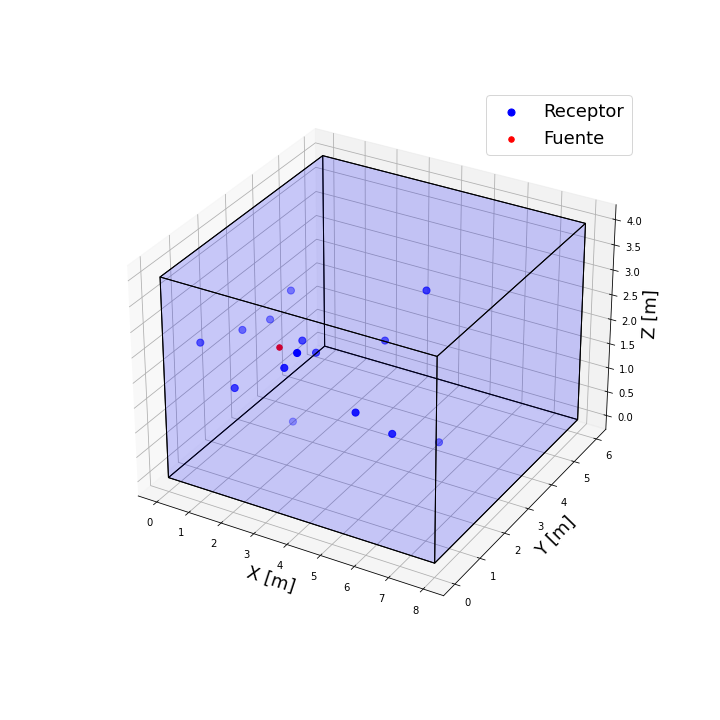
\includegraphics[scale=0.35]{room1.png}
  \caption{Recinto 1}
  \label{fig:sub1}
\end{subfigure}%
\begin{subfigure}{.5\textwidth}
  \centering
  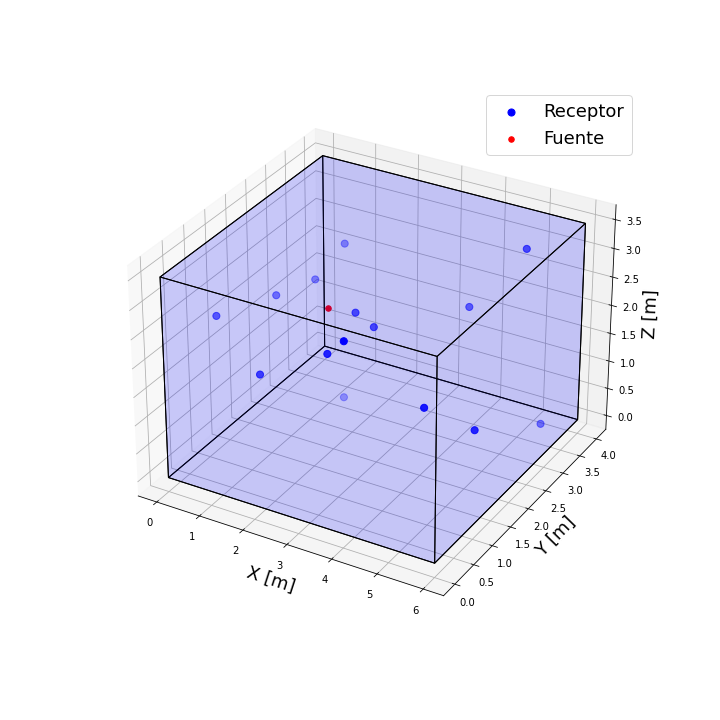
\includegraphics[scale=0.35]{room2.png}
  \caption{Recinto 2}
  \label{fig:sub2}
\end{subfigure}
\caption{Recintos y puntos receptor-fuente generados para la simulación de respuestas al impulso}
\label{fig:recintos}
\end{figure}

Para controlar los demás parámetros que refieren a las condiciones del recinto, se subordina el orden máximo de reflexiones y los coeficientes de absorción a un tiempo de reverberación esperado. Esto es, teniendo un cierto recinto se determina un valor de tiempo de reverberación T60 inicial. Este se utiliza para estimar un valor de un coeficiente de absorción promedio mediante la ecuación de Sabine y también en base a este tiempo se determina el orden de reflexiones necesario para poder representar la reverberación. 
Por último, las posiciones de fuente y receptor se generan aleatoriamente para poder generar diferentes respuestas al impulso a partir de un mismo recinto. De esta manera, los datos que se deben determinar son las dimensiones del recinto, un tiempo de reverberación inicial y la cantidad de respuestas al impulso que se busca generar. 

Con esto, para formar el conjunto de respuestas al impulso generadas de entrenamiento se utiliza el recinto 1 para 3 tiempos de reverberación principales: $0,5 s$ como reverberación baja, $0,75 s$ como reverberación media y $1,0 s$ como reverberación alta. Partiendo de estos tiempos, se generan 30 respuestas al impulso para cada uno, variando aleatoriamente los puntos de fuente y receptor. Esto resulta en un total de 90 respuestas al impulso con tiempos de reverberación de entre aproximadamente $0.5$ segundos a $1.0$ segundos. Para generar las respuestas destinadas a evaluación se realiza el mismo procedimiento pero utilizando el recinto 2 y generando 15 respuestas por cada tiempo de reverberación, formando un total de 45 respuestas al impulso generadas. 

\subsubsection{Respuestas al impulso generadas por aumentación}
Este conjunto se genera partiendo de un subconjunto de respuestas al impulso reales. El proposito de este proceso es partir de un conjunto de impulsos escasos con determinadas características, y generar un conjunto mucho mas grande de respuestas al impulso controlando de manera paramétrica ciertos descriptores acústicos como el tiempo de reverberación $T60$ y la relación directo-reverberado $DRR$, de manera tal que se pueda asegurar un cierto balance en el conjunto conformado \cite{rir_aug}. El proceso de aumentación entonces se divide en dos procesos principales: una alteración de amplitud en la parte temprana de la respuesta al impulso para controlar la relación directo-reverberado, y una alteración de envolvente de caida para controlar el tiempo de reverberación.

Para el primer proceso, a la parte temprana de la respueta al impulso $h_{e}(t)$ se le aplica una ganancia definida por un factor $\alpha$ el cual se calcula para obtener el valor de $DRR$ deseado generando una nueva señal $\tilde{h}_{e}(t)$. Para evitar generar discontinuidades durante el proceso, se aplican ventanas complementarias a la parte temprana obteniendo una parte temprana ventaneada y un residuo ventaneado. A partir de esto, la parte temprana se puede definir segun la ecuación
\ref{eqn:ventaneada}.  

\begin{equation}
\label{eqn:ventaneada}
	h_{e}(t) = \alpha w_{d}(t)h_{e}(t) + [1-w_{d}(t)]h_{e}(t)
\end{equation} 

En donde $w_{d}(t)$ corresponde a una ventana Hann de $5 ms$ de longitud. De esta manera, partiendo de esta ultima definición junto con la expresión del parámetro $DRR$ expresado en la ecuación \ref{eqn:DRR} se plantea un sistema de ecuaciones a partir del cual se puede definir un valor pretendido de $DRR$ y despejar el correspondiente valor de $\alpha$. En la figura \ref{fig:drr_aug} se puede observar una representacion de una parte temprana $h_{e}(t)$, las ventanas aplicadas, el efecto del factor de ganancia $\alpha$ y la nueva señal $\tilde{h}_{e}(t)$ generada. Finalmente, esta parte temprana modificada se concatena con el resto de la respuesta al impulso completando asi el proceso de aumentación referido a la relación directo-reverberado. Se debe tener en cuenta que para tiempos de reveberación cortos, puede ser un problema generar relaciones directo-reverberado demasiado bajas, ya que la energia de la parte tardia ya es de por si muy baja. Para esos casos, se define valores límtes para la ganancia aplicada a la parte temprana.

\begin{figure}[H]
	\centering{}
	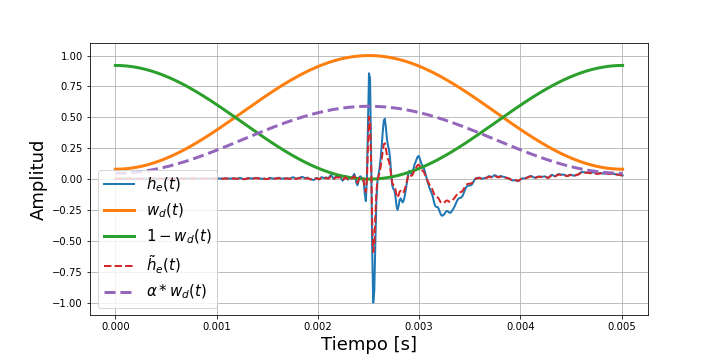
\includegraphics[scale=0.55]{drr_aug.png}
	\caption{Señales involucradas en el proceso de aumentación de DRR}
	\label{fig:drr_aug}
\end{figure}

Luego, para la modificación del tiempo de reverberación $T_{60}$ se trabaja únicamente con la parte tardia de la respuesta al impulso. Esta puede ser modelada como ruido Gaussiano con una caida de´ nivel exponencial dependiente de la frecuencia, sumado a un determinado piso de ruido. Como esta pendiente de caida varia con la frecuencia, se analiza la respuesta al impulso en bandas de tercio de octava para contemplar esta dependencia frecuencial. Este modelo se expresa en la ecuación \ref{eqn:decay_exp}. 
\begin{equation}
\label{eqn:decay_exp}
	h_{m}(t) = A_{m} e^{\frac{-(t-t_{0})}{\tau_{m}}}n(t)u(t-t_{0})+\sigma_{m}n(t)
\end{equation} 
En donde $A_{m}$ es la amplitud inicial, $\tau_{m}$ es la tasa de caida, $\sigma_{m}$ es el nivel del piso de ruido, $n(t)$ es ruido Gaussiano de media cero y desvio estándar unitario, $t_{0}$ es el instante temporal en donde comienza la parte tardia de la respuesta al impulso, $m$ es el indice que indica una sub-banda frecuencial y $u(t)$ es un escalón unitario. En este modelo, el tiempo de reverberación $T_{60}$ se relaciona directamente con el parámetro $\tau$ según la ecuación \ref{eqn:tau60}.

\begin{equation}
\label{eqn:tau60}
	T_{60} = ln(1000)\tau T_{s}
\end{equation}

En donde $T_{s}$ es el período de muestreo. Dado este modelo, se aplican métodos de optimización no lineales para estimar el conjunto de parámetros $\left \{ \hat{A}_{m}; \hat{\tau}_{m}; \hat{\sigma}_{m} \right \}$ que mejor aproximen la envolvente de caida de la respuesta al impulso. Con estos parámetros sumados a la tasa de caida deseada $\tau_{m,d}$ calculada a partir del tiempo de reverberación deseado, se modifica la parte tardia de la respuesta al impulso inicial multiplicandola por una envolvente exponencial creciente o decreciente según corresponda como se muestra en la ecuación  \ref{eqn:aug_tr}.

\begin{equation}
\label{eqn:aug_tr}
	{h_{m}}'(t) = h_{m}(t) e^{-(t-t_{0})\frac{\hat{\tau_{m}}-\tau_{m,d}}{\hat{\tau_{m}}\tau_{m,d}}}
\end{equation}

En donde ${h_{m}}'(t)$ representa a la nueva parte tardia de la respuesta al impulso generada para obtener el tiempo de reverberación deseado. En terminos generales, el proceso consiste en modificar la pendiente de caida para obtener la pendiente de caida deseada por cada banda de frecuencia. Al final, las sub-bandas generadas se suman para obtener el resultado final que contemple todo el espectro de la señal. Hasta aqui este proceso funciona satisfactoriamente cuando se generan tiempos de reverberación menores al de la respuesta al impulso inicial, es decir, siempre que se multiplica la respuesta al impulso por envolventes exponenciales decrecientes. En cambio, cuando se busca generar tiempos de reverberación mayores la envolvente por la que se multiplica la respuesta inicial es creciente, lo que produce una amplificación de la parte tardia de la respuesta al impulso. Esto muchas veces equivale a amplificar el piso de ruido presente en la señal, lo que puede producir pendientes de caida inestables que no se corresponden con el comportamiento propio de la respuesta al impulso ya que no es información del sistema acústico sino simplemente ruido. Para evitar este efecto adverso del proceso de aumentación anteriormente propuesto se debe estimar el piso de ruido de la respuesta al impulso. Esto se realiza a través del método iterativo propuesto por Lundeby et. al. \cite{Lundeby}. Una vez estimado el piso de ruido de la señal, la respuesta final se obtiene haciendo un cross-fade en el inicio del piso de ruido entre la parte tardia generada y una cola reverberante sintética creada a partir de multiplicar ruido Gaussiano con una envolvente exponencial decreciente, utilizando los parámetros previamente calculados. Una explicación mas detallada de este proceso se puede encontrar en el anexo A. 

Para realizar este proceso se determinan limites de relación directo-reverberado y tiempo de reverberación medio. La realción directo-reverberado va desde $-3 \ dB$ a $10 \ dB$ con saltos de $1 \ dB$, lo que se considera una diferencia de nivel promedio acorde a la minima perceptible por el oido humano. Con respecto al tiempo de reverberación, se generan desde $0.1 \ s$ a $1.2 \ s$ para estar dentro del rango de las respuestas al impulso generadas, con un paso de $0.05 s$ basado en estudios previos realizados sobre la minima diferencia perceptible entre tiempos de reverberación \cite{aug_JND}. Una vez obtenido el conjunto de respuestas al impulso aumentadas, se seleccionan aleatoriamente 135 respuestas para equiparar al numero de respuestas al impulso generadas. 

\subsection[Bases de datos de señales de habla]{BASES DE DATOS DE SEÑALES DE HABLA}

Las señales del habla necesarias para formar los pares anecoico-reverberados se obtienen de la librería LibriSpeech \cite{librispeech} la cual consiste en un conjunto de datos que reúne 100 horas de audio correspondientes a lecturas en idioma inglés. Los datos corresponden a programas tipo audiolibros. Las señales poseen bajo nivel de reverberación, y provienen de una aplicación en la cual la inteligibilidad es primordial, lo cual hace que esta base de datos sea adecuada para utilizarse en este trabajo.

\subsubsection{Pre-procesamiento de datos}

Partiendo de audios de voz y respuestas al impulso, el modelo de red neuronal propuesto requiere generar instancias de espectrogramas de magnitud y máscaras ideales para poder entrenarse. Para conseguir esto, se programa una cadena de procesamiento automatizada que realice esta transformación de los datos de entrada. 
En primer lugar se controla la uniformidad de frecuencias de muestreo aplicando las transformaciones de aumentación o decimado cuando sean requeridas. Se decide trabajar con una frecuencia de muestreo de $16000$ muestras por segundo, considerando que se tratan con señales de voz que concentran su información por debajo del límite de representación frecuencial de $8000 Hz$ impuesto por esta decisión. 
Luego, los audios de voz se convolucionan con las respuestas al impulso para formar pares de señales con y sin reverberación. El resultado de la convolución se recorta para descartar el retardo generado por la convolución, haciendo que los pares de señales sean sincrónicas. Luego, se toman ventanas rectangulares de $32640$ muestras, lo que equivale a segmentos de audio de $2,04$ segundos para la frecuencia de muestreo utilizada. Lo siguiente es aplicar la transformada de corto término de Fourier tanto a la señal limpia como a la señal convolucionada. La transformada se aplica con una ventana de $512$ muestras y un salto de $128$ muestras lo cual equivale a un solapamiento del $75\%$. Esto permite la correcta reconstrucción de la señal al antitrasformar. Se obtienen espectrogramas complejos, a los cuales se les calcula la magnitud, descartando la información de fase. Además, se aplica una normalización para acotar el dominio en valores que sean convenientes para el algoritmo de  aprendizaje posterior. Con las magnitudes de los espectros anecoicos y reverberados, se calculan máscaras de amplitud ideales y luego se comprimen aplicando una función tangencial hiperbólica para la cual se definen los parámetros $Q=1$ y $C=0,5$. Finalmente, las instancias finales de este proceso son en el espectro de magnitud de la señal con reverberación (que corresponde a la variable de entrada de la red neuronal) y la máscara de magnitud ideal comprimida (que corresponde a la salida de la red, es decir, el objetivo que el modelo busca estimar). Ambas instancias tienen las mismas dimensiones, que corresponden a $256$ cuadros temporales y $257$ valores posibles de frecuencia (se conserva solo la parte positiva del espectro frecuencial simétrico). Por último, se descartan los puntos correspondientes al valor máximo de frecuencia. Esto se realiza para obtener dimensiones finales de $256x256$ lo cual facilita el proceso de compresión y expansión de los espectros al ser dimensiones múltiplos de $2$. Se descarta la frecuencia más alta ya que por la característica de la fuente  no contendrá información crucial para la representación.  

Cabe destacar que debido a este preprocesamiento aplicado, a la hora de evaluar el modelo se deberán aplicar una serie de procesos previos sobre el audio a procesar. Mas precisamente, se deberá segmentar el audio y obtener espectros de magnitud de la STFT respetando los mismos parámetros que en el preprocesamiento. Luego, como la salida de la red es una máscara de amplitud comprimida, se debe descomprimir esta máscara, aplicarla sobre el espectro reverberado y luego combinar el espectro de amplitud modificado resultante con la fase original de la señal para poder finalmente obtener la información de audio de salida a través de la aplicación del algoritmo de Griffin-Lim.  


\subsection[Modelo propuesto]{MODELO PROPUESTO}

El modelo propuesto se basa en una arquitectura de red neuronal completamente convolucional tipo 'autoencoder' inspirada en el trabajo de Ernst et. al.\cite{FCN}. Más precisamente, un autoencoder es una estructura que tiene como objetivo aprender niveles de representación de la información de entrada, para luego poder reconstruir una instancia similar descartando la información no deseada o considerada "ruido". En este caso, la señal no deseada corresponde a la reverberación. El esquema básico del algoritmo se puede observar en la figura \ref{fig:autoencoder}, donde la variable $x$ representa a las variables de entrada, e $y$ representa la variable de salida. 

\begin{figure}[H]
	\centering{}
	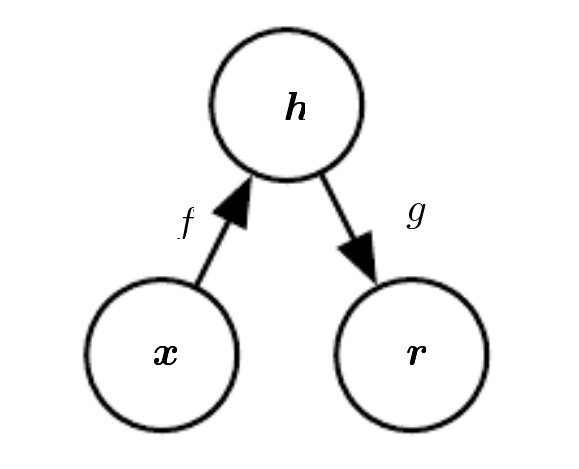
\includegraphics[scale=0.3]{autoencoder.png}
	\caption{Estructura general de un autoencoder.}
	\label{fig:autoencoder}
\end{figure}

El esquema se compone de tres partes fundamentales: 
\begin{itemize}
\item Una función de codificación $f$ en donde las dimensiones de la variable de entrada se comprimen y las características más relevantes son aprendidas. Esta función realiza el mapeo de la variable de entrada al espacio latente. 
\item Un espacio latente $h$ (o espacio de representación), en donde se concentran las representaciones internas aprendidas a partir de la compresión de la variable de entrada. 
\item Una función de decodificación en donde se aplica el proceso inverso que en la codificación, expandiendo las dimensiones tomadas del espacio latente para formar una representación que minimice el error de reconstrucción. 

\end{itemize}

El sistema propuesto consiste en la estimación del espectro de la señal anecoica a partir del espectro de la señal reverberada. Para conseguirlo, en lugar de hacer un mapeo directo entre ambos espectros, se opta por estimar una máscara de amplitud. Se decidió trabajar con máscaras ya que estudios previos demostraron que con este método se obtienen mejores resultados que realizando estimaciones de mapeos directos entre dos espectros. Para trabajar con espectros, las señales de entradas se transforman al dominio temporal-frecuencial a partir de la transformada de Fourier de corto término. Se utiliza una ventana temporal de 512 muestras, con un solapamiento del 75\%. 
La estructura de red neuronal utilizada consiste en una U-NET con conexiones de saltos, inspirada inicialmente en \cite{FCN}. Este tipo de estructuras consiste en tomar mapas bidimensionales de entrada y a partir de la aplicación sucesiva de capas convolucionales con valores de salto mayor a 1, reducir la dimensionalidad del mismo e ir aumentando el número de filtros utilizados por la capa convolutiva. Un esquema básico de está estructura se puede ver en la figura \ref{fig:unet}, en donde se puede ver que las dimensiones de las capas siguen una forma de 'U', lo cual le da el nombre a estas estructuras.

\begin{figure}[H]
	\centering{}
	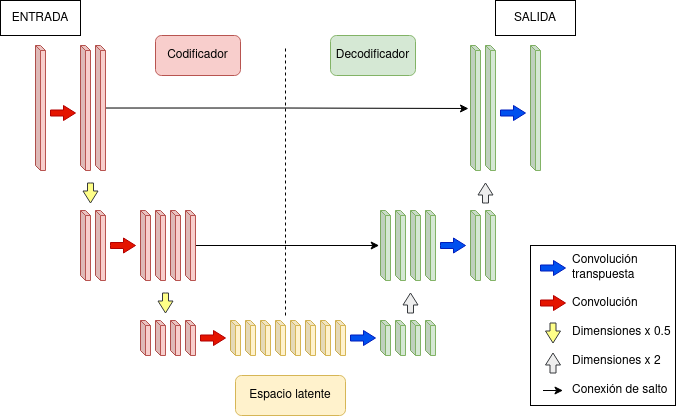
\includegraphics[scale=0.3]{unet.png}
	\caption{Esquema básico de una red tipo 'U-NET'.}
	\label{fig:unet}
\end{figure}

A medida que se avanza en el modelo, el tamaño del espectro de entrada va disminuyendo y la cantidad de filtros utilizados va aumentando. Esta primera parte se puede pensar como un codificador, ya que el sistema esta tomando información del espectro de manera jerárquica.  Este proceso se realiza sucesivamente hasta que la imagen de entrada alcanza una dimensión de 1x1. Luego, prosigue una etapa de decodificación en la cual se aplica el proceso inverso. Esto es, la dimensión del espectro se va aumentando con capas convolutivas transpuestas de saltos mayores a 1, y la cantidad de filtros utilizados va disminuyendo. Esto se repite hasta que las dimensiones del espectro sean las mismas que tenía a la entrada del codificador. Mediante este esquema de U-NET y el efecto del cuello de botella de las dimensiones, se consigue que la estimación de cada pixel de la imagen resultante esté condicionado por todos los pixeles que componen la imagen de entrada. Se puede decir entonces que la estimación de cada punto del espectro final depende de todo el espectro de entrada, y no solo de una región determinada. 

Para poder pasar información de manera más directa desde el decodificador hacia el codificador, se implementan conexiones de salto. La conexión de salto consiste en concatenar la salida de una capa del codificador con una capa del decodificador. Para poder hacerlo, la dimensión de concatenación (en este caso, las dimensiones del espectrograma) deben ser las mismas. De esta manera se logran decodificaciones más precisas. 


Una representación gráfica del modelo final implementado se puede apreciar en la figura \ref{fig:modelo}. En cada capa se indican tres valores, donde el primero representa la dimension temporal, el segundo la dimension frecuencial y el tercero el numero de canales. En las primeras capas, las dimensiones se reducen a la mitad en cada instancia debido al uso de un desplazamiento de paso 2 en los filtros convolucionales, lo que realiza la compresión de la información. En las capas subsiguientes, las dimensiones sufren el efecto contrario hasta volver a obtener las dimensiones originales. Este tipo de estructura tiende a perder información importante de bajo nivel durante el proceso de compresión. Como por lo general las variables de entrada y de salida comparten información estructural, se puede mejorar el funcionamiento de estas estructuras implementando conexiones entre las capas del codificador y el decodificador. Esto quiere decir que los mapas de características de las capas que conforman el codificador se van a concatenar directamente con los mapas de características en el decodificador, es decir, la salida de la capa $i$ se concatena con la salida de la capa $N-i$ donde $N$ es el número de capas. Estos saltos evitan que las activaciones pasen por el cuello de botella permitiendo la propagación de esta información estructural que estas estructuras tienden a perder. 

\begin{figure}[H]
	\centering{}
	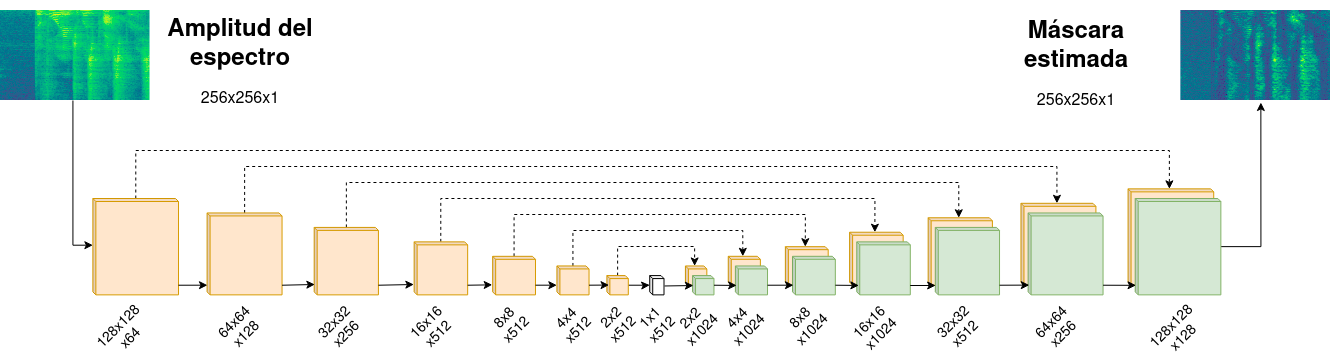
\includegraphics[scale=0.35]{modelo_red.png}
	\caption{Modelo de red neuronal convolucional implementado}
	\label{fig:modelo}
\end{figure}

De esta forma, el modelo realiza una compresión de los datos de entrada, buscando minimizar el error en la reconstrucción al comparar con las instancias que se le presentan como objetivo. 
Para este caso particular, las entradas del modelo son espectrogramas, es decir, valores en el dominio tiempo-frecuencia. Las dimensiones del espectrograma de entrada son comprimidas hasta llegar a dimensiones de $1x1$ y luego son expandidas nuevamente, lo que produce un aumento de los campos perceptivos que permite propagar información global tanto en tiempo como en frecuencia. Esto significa que el cómputo de cada pixel de salida se verá influenciado por la totalidad del espectrograma de entrada. Estudios previos demostraron que la estimación directa de espectros, o lo que es equivalente, el mapeo frecuencial-temporal genera resultados menos precisos comparado con aquellos modelos que en lugar de estimar espectros estiman máscaras espectrales\cite{mask_vs_map}. Por esto, las entradas del modelo son espectrogramas correspondientes a señales con reverberación, y las salidas u objetivos son máscaras de amplitud previamente calculadas en una etapa de preprocesamiento. 

\subsection[Especificaciones de la arquitectura implementada]{ESPECIFICACIONES DE LA ARQUITECTURA IMPLEMENTADA}

Como se indicó anteriormente, esta arquitectura se basa en el entrenamiento de un modelo completamente convolucional. Sin embargo, la etapa de codificación y decodificación requieren evaluar ciertos detalles a la hora de su implementación. 

En la etapa de codificación, la primera capa consiste en una capa convolucional utilizando una activación del tipo Leaky-Relu con una pendiente de $0,2$. Se escoge esta activación por sobre la rectificación lineal debido a que es favorable frente al problema de desvanecimiento de gradiente, lo cual puede ser un problema al trabajar con una arquitectura de red tan profunda. Luego, las seis capas subsiguientes son también capas convolucionales con la misma función de activación pero con el agregado de que implementan normalización por lotes. Finalmente, la última capa de esta etapa es convolucional con normalización por lotes y función de activación ReLU. 

En la etapa de decodificación es importante tener en cuenta que el tamaño de los campos perceptivos de las capas deben ser un múltiplos enteros del tamaño de salto para que no se produzcan artefactos indeseados durante el proceso inverso al cuello de botella que ocurre al utilizar capas deconvolutivas con tamaño de salto mayor a $1$. Sin embargo, aun teniendo esto en consideración, las capas de deconvolución pueden generar artefactos indeseados. En lugar de utilizar capas convolutivas se opta por implementar una combinación de dos capas consecutivas: en primer lugar una capa que aumente las dimensiones del espectrograma generando nuevos puntos a partir de una interpolación entre los valores mas cercanos, y luego una capa convolutiva. De esta manera se obtiene el efecto del aumento de dimensiones junto con el análisis convolutivo. Esta deconvolución se combina con un drop-out del 50\% y una función de activación ReLU en las primeras tres capas del decodificador. Luego, continuan 4 capas idénticas pero omitiendo el drop-out. Finalmente, la última capa del decodificador que a la vez es la capa de salida de la red consiste también en una deconvolución sin drop-out pero utilizando una función de activación tangencial, lo que significa que los valores de salida estarán acotados en el intervalo $[-1, 1]$.
En todas las capas convolucionales y deconvolucionales se utiliza un tamaño de filtro de $6x6$ y un tamaño de salto igual a $2$. 
Finalmente, la función de costo utilizada para evaluar las predicciones realizadas por el modelo frente a las máscaras ideales en la salida es el error cuadrático medio (MSE) el cual se expresa en la ecuación \ref{eqn:mse} y para la optimización se utilizó el algoritmo de estimación adaptativa de momento (ADAM) \cite{adam} con un valor de tasa de aprendizaje de $0,001$. 

\begin{equation}
\label{eqn:mse}
	L_{MSE} = \sum_{i=1}^{N-1}\overline{(M_{i}(t,f) - \hat{M}_{i}(t,f))^{2}} 
\end{equation}

\subsection[Evaluación del modelo]{EVALUACIÓN DEL MODELO}
En este trabajo se ponen a prueba cuestiones relativas al manejo, generación y aumentación de datos utilizados para el entrenamiento del modelo. Las evaluaciones se diferencian entre combinaciones entre datos simulados o reales, y en el ordenamiento de la complejidad de los datos durante el entrenamiento. 

\subsubsection{Combinaciones de bases de datos}
En primer lugar, como se cuenta con respuestas al impulso reales, simuladas o generadas, y aumentadas, se prueban combinaciones de estos datos a la hora de formar los diferentes conjuntos de entrenamiento y validacion. Es decir, se entrena el modelo utilizando un determinado conjunto, y luego se evalua su funcionamiento sobre el total de los conjuntos. Esto desemboca en 3 pruebas, en donde los conjuntos de entrenamiento y evaluación quedan determinados segun la tabla \ref{tab:pruebas}. 


\begin{table}[H]
\caption{Configuración del primer conjunto de pruebas.}
\centering
\begin{tabular}{|c|c|c|c|}
\hline
                          & \textbf{Prueba 1}                                                       & \textbf{Prueba 2}                                                       & \textbf{Prueba 3}                                                       \\ \hline
Conjunto de entrenamiento & Reales                                                                  & Generadas                                                               & Aumentadas                                                              \\ \hline
Conjuntos de evaluacion   & \begin{tabular}[c]{@{}c@{}}Reales\\ Generadas\\ Aumentadas\end{tabular} & \begin{tabular}[c]{@{}c@{}}Reales\\ Generadas\\ Aumentadas\end{tabular} & \begin{tabular}[c]{@{}c@{}}Reales\\ Generadas\\ Aumentadas\end{tabular} \\ \hline
\end{tabular}
\label{tab:pruebas}
\end{table}

Luego, se evalua el rendimiento del modelo propuesto al utilizar combinaciones de conjuntos en la etapa de entrenamiento. Como el objetivo principal es lograr extender la variedad presente en las respuestas al impulso reales, las combinaciones propuestas consisten en combinar las respuestas reales con las generadas y aumentadas como se indica en la tabla \ref{tab:pruebas_combinadas}. 

\begin{table}[H]
\caption{Configuración del segundo conjunto de pruebas.}
\centering
\begin{tabular}{|c|c|c|c|}
\hline
                          & \textbf{Prueba 1}                                                       & \textbf{Prueba 2}                                                       & \textbf{Prueba 3}                                                                   \\ \hline
Conjunto de entrenamiento & \begin{tabular}[c]{@{}c@{}}Reales \\ + \\ Aumentadas\end{tabular}       & \begin{tabular}[c]{@{}c@{}}Reales\\  + \\ Generadas\end{tabular}        & \begin{tabular}[c]{@{}c@{}}Reales \\ + \\ Aumentadas \\ + \\ Generadas\end{tabular} \\ \hline
Conjuntos de evaluacion   & \begin{tabular}[c]{@{}c@{}}Reales\\ Generadas\\ Aumentadas\end{tabular} & \begin{tabular}[c]{@{}c@{}}Reales\\ Generadas\\ Aumentadas\end{tabular} & \begin{tabular}[c]{@{}c@{}}Reales\\ Generadas\\ Aumentadas\end{tabular}             \\ \hline
\end{tabular}
\label{tab:pruebas_combinadas}
\end{table}

\subsubsection{Ordenamiento de los datos durante el entrenamiento}

Por otro lado, se evalua la influencia del orden de complejidad con el que las instancias de entrenamiento se le presentan a la red, siguiendo los lineamientos de la técnica de aprendizaje por curriculum. En este caso se considera que una instancia de audio es más compleja de dereverberar cuando posee un mayor tiempo de reverberación, debido a que esto equivale a una mayor distorsión de la señal original que se quiere recuperar. Entonces, se decide comparar el rendimiento del sistema final al ser entrenado con instancias en las cuales los tiempos de reverberación esten ordenados en forma creciente (curriculum), ordenados en forma decreciente (anti-curriculum) y ordenados aleatoriamente. 

Para esta evaluación del orden de los datos en el entrenamiento, es necesario generar un conjunto de datos anecóicos-reverberados de manera controlada, asegurando una distribución homogenea de los tiempos de reverberación presentes en el conjunto final. Para conseguir esto se decide conformar el conjunto de datos a partir de respuestas al impulso aumentadas, ya que estas se pueden generar controlando paramétricamente el tiempo de reverberación medio y la relación directo-reverberado. Se busca cubrir el rango de tiempo de reverberación medio desde $0.1 \ s$ hasta $3.5 \ s$ con variaciones de relación directo-reverberado desde $-10 \ dB$ a $10 \ dB$. 

\newpage
\section{Resultados}


\subsection{Armado de datos}

\subsubsection{Variables del sistema}

\subsection{Metricas}


\newpage
\section{Conclusiones}
A lo largo de este trabajo se implementó un algoritmo de aprendizaje profundo para la tarea de dereverberación de señales de habla. Se utilizó una estructura de tipo autoencoder, la cual se entrenó para estimar máscaras de amplitud que al aplicarse sobre un espectro reverberado generen un espectro dereverberado, que luego de procesarse pueda desembocar en información de audio dereverberado. Particularmente se estudió la influencia del manejo de datos para el entrenamiento de este algoritmo, manipulando y generando respuestas al impulso de diversas maneras. 
\newpage
\section[Lineas futuras de investigación]{CAPÍTULO 7:$\ \ \ \ $LINEAS FUTURAS DE INVESTIGACIÓN} 

La dereverberación del habla a partir de la estimación de máscaras de amplitud demostró ser un proceso eficaz pero limitado. Pueden obtenerse mejoras expandiendo el procesamiento para que se consideren también las componentes complejas de la STFT, es decir, realizar la dereverberación en amplitud y fase. Esto se podría conseguir estimando máscaras complejas o bien estimando máscaras independientes para magnitud y fase. Por otro lado, en este enfoque se procesa de la misma manera la totalidad del espectro. Sabiendo que la reverberación aporta más energía en bajas frecuencias, podría segmentarse el espectro en bandas y procesar cada banda con configuraciones diferentes. 
De manera más general, también podrían aprovecharse dependencias temporales presentes en la reverberación introduciendo capas recurrentes dentro de la estructura de capas convolucionales. 

Otro aspecto a considerar es el referido a las métricas utilizadas tanto para el entrenamiento como para la evaluación de los modelos. Se deben analizar y proponer nuevas métricas que se correlacionen de manera directa con la percepción auditiva de la tarea de dereverberación \cite{CDPAM}. De esta forma el entrenamiento se realizará en pos de una mejora en la percepción auditiva de los resultados, y los resultados de las evaluaciones podrán ser utilizados para tomar decisiones que mejoren la calidad del proceso de dereverberación de manera consistente y objetiva.

Respecto al proceso de aumentación, es de interés tener un cierto control sobre el perfil frecuencial de tiempo de reverberación con el que se generan las respuestas al impulso aumentadas. En este trabajo, estas respuestas al impulso siguen las mismas relaciones interfrecuenciales que las respuestas al impulso de las que parten, generando el mismo perfil de tiempo de reverberación pero desplazado. Una mayor diversidad de respuestas podría conseguirse si se logra controlar también la forma general de la curva de tiempo de reverberación. 

Perfeccionar las técnicas de aumentación de respuestas al impulso podría llevar en un futuro a la creación de un corpus de datos de dominio libre destinado específicamente al desarrollo de sistemas de dereverberación del habla, estandarizando y dando acceso a los mismos datos de entrenamiento y evaluación para todos los estudios de dereverberación. Generar esta base de datos de acceso libre puede asegurar que exista una correcta comparación entre las soluciones propuestas por diferentes trabajos, de forma tal que cada resultado logre contribuir de manera objetiva a la mejora general de las técnicas de dereverberación. 
\newpage

\printbibliography[heading=bibintoc,title={Bibliografía}]


\appendix
\clearpage
\addappheadtotoc
%\appendixpage

\section[Aumentación de tiempo de reverberación]{ANEXO A:$\ \ \ \ $AUMENTACIÓN DE TIEMPO DE REVERBERACIÓN}

El proceso de aumentación de respuestas al impulso puede realizarse tomando como parámetros del proceso ciertos descriptores acústicos como el tiempo de reverberación $TR_{60}$. Esto es, partiendo de una respuesta al impulso con un $TR_{60}$ determinado, se busca generar nuevas respuestas al impulso cuyo $TR_{60}$ pueda ser controlado paramétricamente para ocupar de manera homogénea y balanceada un rango de valores de interés. 
El $TR_{60}$ se relaciona directamente con la forma de la envolvente de caída de nivel exponencial presente en la parte tardía de las respuestas al impulso. El proceso de aumentación equivale a modificar esta pendiente de caída, multiplicando la señal original por una nueva envolvente que produzca el efecto deseado en la envolvente resultante. Los pasos a seguir para realizar este proceso son: 

\begin{itemize}
  \item Acondicionamiento de la respuesta al impulso de entrada.
  \item Filtrado por bandas de octava o bandas de tercio de octava.
  \item Estimación de piso de ruido.
  \item Estimación de envolvente de caída.
  \item Sintetizar una señal aplicando la envolvente estimada con piso de ruido cero a una señal de ruido Gaussiano. 
  \item Realizar el cross-fade entre la señal sintetizada y la señal original en el punto inicial del piso de ruido.
  \item Aumentación de la envolvente de caída multiplicando la señal por la correspondiente envolvente exponencial creciente/decreciente.
  \item Suma de las sub-bandas para obtener la señal resultante en su espectro completo.
  \item Integración de la parte tardía aumentada con la parte temprana de la respuesta al impulso inicial.
\end{itemize} 	

A continuación se explica cada paso del algoritmo con mayor profundidad.
%Acondicionamiento
En primer lugar, se define una determinada frecuencia de muestreo y profundidad de bits para trabajar con la señal de entrada, en este caso una respuesta al impulso real. Una vez asegurada la homogeneidad de estas características, la señal se normaliza para trabajar en un rango de amplitud acotado en el intervalo $[-1,1]$ y luego se separa la parte temprana de la parte tardía de la respuesta al impulso. Esto último se realiza aplicando ventanas temporales de acuerdo a lo que indican las ecuaciones \ref{eqn:early} y \ref{eqn:late}, utilizando una ventana de tolerancia de $t_{0} = 2.5 ms$. Para los pasos siguientes se trabaja únicamente modificando la parte tardía, y la parte temprana se almacena para ser utilizada en el paso final a la hora de reconstruir la respuesta completa. En la figura \ref{fig:impulso_entrada} se  muestra la respuesta al impulso desde la que se parte, distinguiendo la descomposición temporal de la misma y luego la parte tardía de la respuesta al impulso aislada con la que se va a trabajar durante el proceso.

\begin{figure}[H]
	\centering{}
	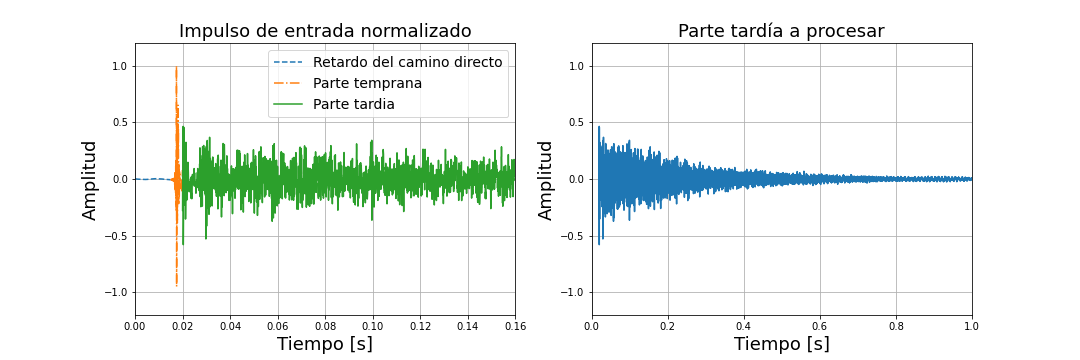
\includegraphics[scale=0.45]{impulso_entrada.png}
	\caption{Descomposición de la respuesta al impulso a procesar durante la aumentación temporal}
	\label{fig:impulso_entrada}
\end{figure}

Luego, el siguiente paso consiste en descomponer la señal en bandas de octava o tercios de octava. En esta demostración se trabaja con bandas de octava desde $125 \ Hz$ hasta $4000 \ Hz$ teniendo en cuenta que se trabaja con una frecuencia de muestreo de $16000$ muestras por segundo. Es necesario trabajar en sub-bandas frecuenciales para contemplar la dependencia del tiempo de reverberación con la frecuencia, y mantener esa característica en las señales a generar en este proceso. Para conseguir esta descomposición en sub-bandas frecuenciales se crea un banco de filtros. El mismo se compone de filtros Butterworth que van siendo creados a partir de las frecuencias centrales que se quiera obtener en cada banda. El proceso consiste en crear filtros pasa-banda para generar una banda de paso alta y una banda de paso baja. Luego, se toma la banda de paso alta y se la vuelve a dividir en banda de paso alta y baja aplicando un nuevo par de filtros pasa-banda. Esto se repite hasta completar todas las frecuencias de corte necesarias. De esta forma se obtiene el prototipo IIR de cada filtro que compone el banco de filtros. Una vez obtenido esto, se crean respuestas de tipo FIR para cada filtro a través de pasar un impulso ideal por cada filtro. En la figura \ref{fig:banco_filtros} se puede observar la respuesta en frecuencia del banco de filtros. Un detalle importante a considerar es que la suma del efecto de todos los filtros es unitaria para todo el rango frecuencial analizado, siendo esta una característica necesaria para poder descomponer la señal en bandas y luego re-componer la señal sumando las bandas sin generar ningún tipo de distorsión en el proceso. Para lograr esto, los coeficientes de los filtros deben ser elevados al cuadrado (lo que equivale poner dos filtros en cascada) para lograr que en las intersecciones entre los filtros la suma de amplitud sea unitaria (en la frecuencia de corte se genera una caída de 6 dB en lugar de los 3 dB que presentaria un filtro Butterworth simple). 

\begin{figure}[H]
	\centering{}
	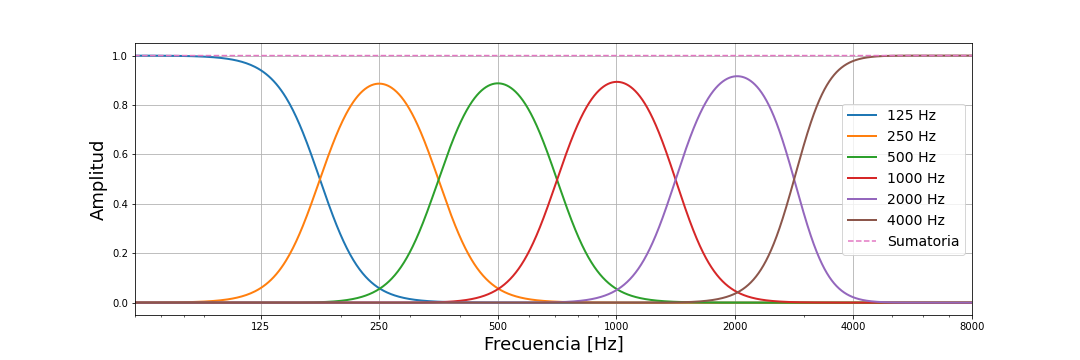
\includegraphics[scale=0.45]{banco_filtros.png}
	\caption{Banco de filtros Butterworth}
	\label{fig:banco_filtros}
\end{figure}

A partir de aplicar este banco de filtros, la señal de entrada se descompone en 6 sub-bandas como se muestra en la figura \ref{fig:sub_bandas}. En este gráfico se puede apreciar como la pendiente de caída varia según la banda de frecuencia que se observa. Todos los procesos subsiguientes se aplican de manera independiente para cada banda, y luego al final las bandas se suman para volver a tener una señal correspondiente al espectro completo original. De ahora en adelante, por una cuestion de simplicidad se muestran los gráficos pertenecientes a la banda de $1000 Hz$ de manera ilustrativa.

\begin{figure}[H]
	\centering{}
	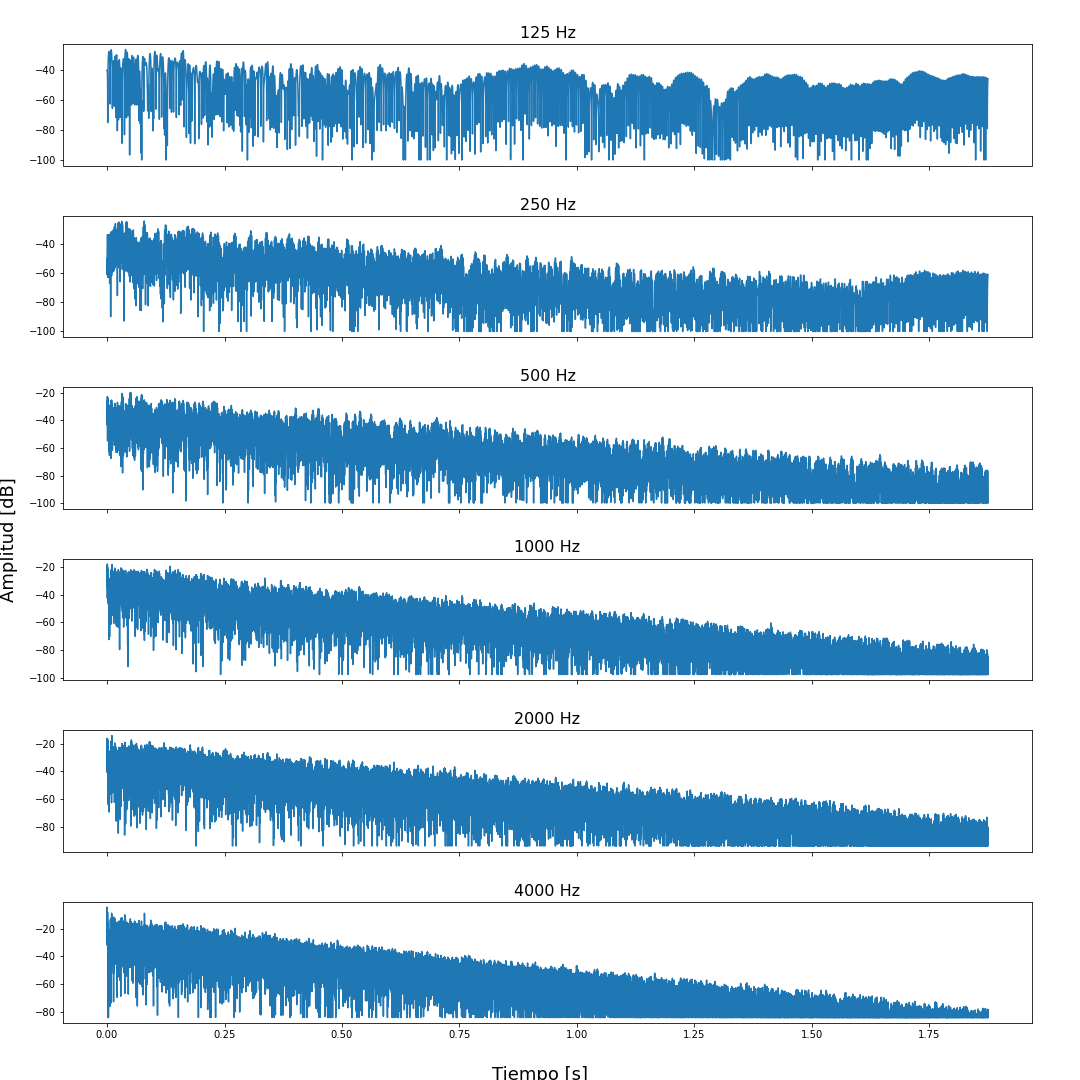
\includegraphics[scale=0.45]{sub_bandas.png}
	\caption{Sub-bandas obtenidas luego de aplicar el banco de filtros}
	\label{fig:sub_bandas}
\end{figure}

El paso siguiente consiste en determinar el piso de ruido de la señal. Detectar el piso de ruido permite asegurar que el método de aumentación no amplifique ruido cuando se busca obtener un tiempo de reverberación mayor al inicial propio de la respuesta al impulso de entrada. Para determinar el punto donde predomina el ruido en la respuesta al impulso se utiliza el método iterativo de Lundeby \cite{Lundeby}. El mismo consta de los siguientes pasos: 

\begin{enumerate}
\item La respuesta al impulso al cuadrado es promediada en intervalos de tiempo locales de entre $10 \ ms$ y $50 \ ms$ para obtener una curva 'suavizada', es decir, disminuir las variaciones instantaneas sin perder las pendientes cortas.
\item Se hace una primera estimacion del piso de ruido. Para hacerlo se toma el segmento correspondiente al último $10\%$ de la respuesta al impulso.
\item La pendiente de caída se estima aplicando una regresión lineal sobre el intervalo de tiempo que contiene la respuesta entre el pico de $0 \ dB$ y el primer intervalo $5-10 \ dB$ por encima del ruido de fondo.
\item Se determina un punto de cruce provisorio en la intersección entre la pendiente de caída estimada y el nivel de piso de ruido.
\item Se obtiene un nuevo intervalo de tiempo de acuerdo a la pendiente calculada, de manera que haya entre $3$ y $10$ intervalos por cada $10 \ dB$ de caída
\item Se vuelve a promediar localmente el impulso al cuadrado de acuerdo al nuevo intervalo temporal calculado previamente 
\item Se estima el ruido de fondo nuevamente. El segmento a evaluar debe corresponder a $5-10 \ dB$ luego del punto de cruce (siguiendo la curva estimada previamente), o bien, un minimo del $10\%$ de la señal total (en el caso de tener que optar por el $10\%$ de nuevo, el resultado seria el mismo que antes, y el punto encontrado previamente seria el definitivo).
\item Se estima la pendiente de caída para un rango dinámico de entre $20 \ dB$ y $10 \ dB$, empezando desde un punto $5-10 \ dB$ por encima del nivel de ruido.
\item Se encuentra un nuevo punto de cruce.
\item Los pasos 7-9 se repiten hasta que el valor del piso de ruido converja, tolerando un maximo de 6 iteraciones.
\end{enumerate}

El paso siguiente es estimar la pendiente paramétrica que mejor se aproxime a la pendiente de caída real. La estimación se basa en el modelo de la ecuación \ref{eqn:decay_exp}. Por lo tanto, los parámetros que se busca estimar son la amplitud inicial, la tasa de caída y el nivel de piso de ruido. La estimación se realiza aplicando un algoritmo de ajuste no lineal por cuadrados mínimos. El resultado de la estimación para la banda de $1000 Hz$ se muestra en la figura  \ref{fig:estimacion_parametrica}.

\begin{figure}[H]
	\centering{}
	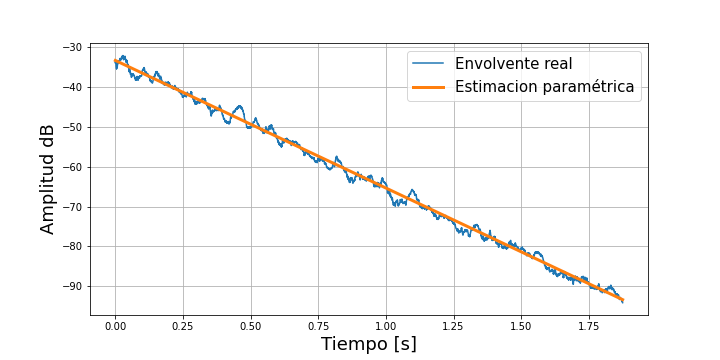
\includegraphics[scale=0.45]{estimacion.png}
	\caption{Estimación paramétrica de la pendiente de caída.}
	\label{fig:estimacion_parametrica}
\end{figure}

Con estos parámetros estimados se genera una nueva envolvente de caída pero llevando el nivel de piso de ruido a cero, y se aplica esta envolvente sobre una señal de ruido Gaussiano de media cero y desvío estándar unitario. Con esta señal sintética y la señal original se hace una transición cruzada en el punto estimado del piso de ruido. De esta manera se elimina el ruido de la señal original, reemplazádolo por la caída exponencial determinada por la envolvente paramétrica.  En la figura \ref{fig:recorte_ruido} se puede observar como se extiende la respuesta luego del punto de inicio del piso de ruido de la señal original.

\begin{figure}[H]
	\centering{}
	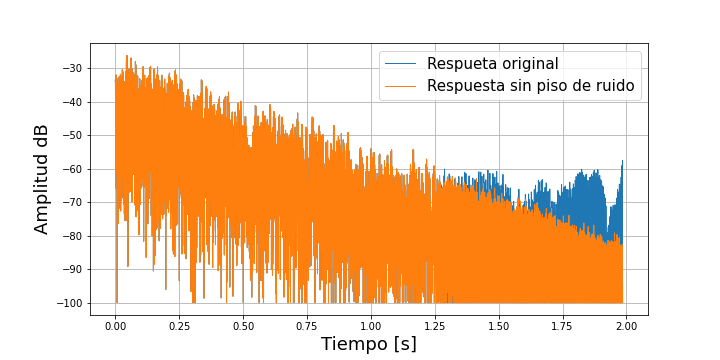
\includegraphics[scale=0.45]{recorte_ruido.png}
	\caption{Respuesta original y extendida sin piso de ruido.}
	\label{fig:recorte_ruido}
\end{figure}
  
Finalmente, teniendo las bandas extendidas y habiéndose eliminado el piso de ruido, se prosigue con el proceso de aumentación del tiempo de reverberación para cada sub-banda, multiplicando cada respuesta por la correspondiente envolvente exponencial creciente o decreciente según corresponda, para obtener la envolvente de caída necesaria para generar el tiempo de reverberación deseado, como se indica en la ecuación \ref{eqn:aug_tr}. Un ejemplo del resultado de la aumentación sobre una sub-banda de frecuencia se muestra en la figura \ref{fig:banda_aumentada}, en donde el tiempo de reverberación objetivo es menor que el tiempo de reverberación de la respuesta original, por lo cual la pendiente aumentada resulta mas atenuada que la pendiente original. 

\begin{figure}[H]
	\centering{}
	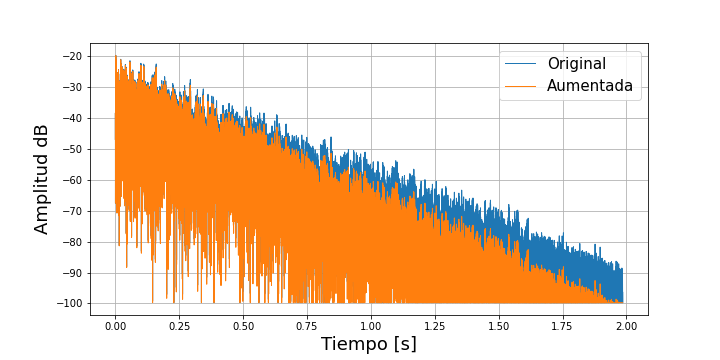
\includegraphics[scale=0.45]{banda_aumentada.png}
	\caption{Aumentación del tiempo de reverberación alterando la envolvente de caída original.}
	\label{fig:banda_aumentada}
\end{figure}

Una vez realizada la alteración de la envolvente de caída para todas las bandas frecuenciales, estas se suman para conformar nuevamente la parte tardía de la respuesta al impulso de espectro completo. El paso final consiste en concatenar los segmentos de la respuesta al impulso original que no fueron alterados, es decir, el delay del camino directo y la parte temprana de la respuesta. Con esto, el proceso de aumentación termina, y se obtiene como resultado una nueva respuesta al impulso con el tiempo de reverberación deseado. En la figura \ref{fig:salida_aumentacion_tr} se muestra la respuesta al impulso original comparada con la nueva respuesta generada a partir del proceso anteriormente descrito. 

\begin{figure}[H]
	\centering{}
	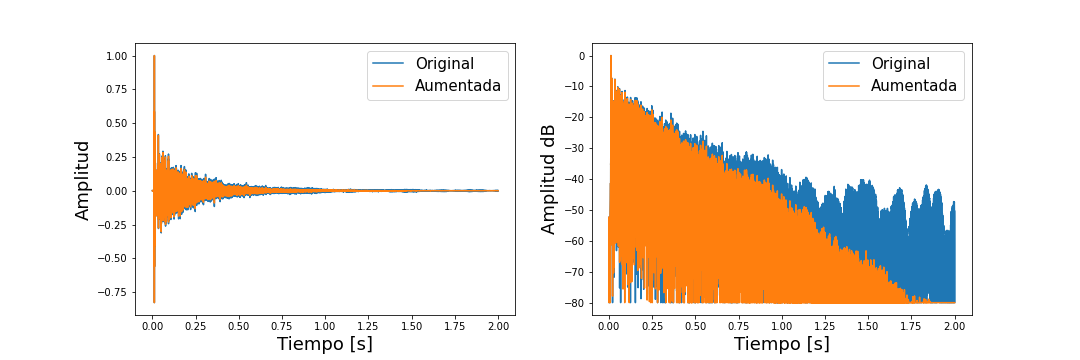
\includegraphics[scale=0.45]{tr_aug.png}
	\caption{Resultado del proceso de aumentación del tiempo de reverberación de una respuesta al impulso}
	\label{fig:salida_aumentacion_tr}
\end{figure}









\end{document}
